%!TEX encoding = UTF-8 Unicode 
%!TEX TS-program = pdflatex

% Optimization Project: Biscuit Optimizer
% Roberto Basla
% Politecnico di Milano
% A.Y. 2021/2022

\documentclass[a4paper,12pt,english]{article} 
\usepackage[utf8]{inputenc}
\usepackage{babel}
\usepackage[T1]{fontenc}
\usepackage{indentfirst}
\usepackage{upquote}
\usepackage{subcaption}
\usepackage{float}
\usepackage{hyperref}
\usepackage{graphicx} 
\usepackage{amsmath}
\usepackage{amssymb}
\usepackage{enumitem}
\usepackage{listings}

\graphicspath{{./img/}}
\hypersetup{%
	colorlinks=true,% hyperlinks will be coloured
	linkcolor=black,% hyperlink text will be green
	urlcolor=blue
}

\pagestyle{plain} 
\author{Roberto Basla -- Politecnico di Milano}
\date{Politecnico di Milano \\
	School Of Industrial and Information Engineering  \\
	Computer Science and Engineering \\
	A.Y. 2021/2022}
\title{Optimization project: Biscuit Optimizer}

\fboxsep=1mm %padding thickness
\fboxrule=0.1mm %border thickness

\begin{document}	
	\maketitle
	\newpage
	
	\tableofcontents
	\newpage
	
	% Optimization Project: Biscuit Optimizer
% Roberto Basla
% Politecnico di Milano
% A.Y. 2021/2022

\section{Introduction}
This document reports the project developed for the Optimization course at Politecnico di Milano. Input data, models and solutions are available at the GitHub repository \href{https://github.com/rb-sl/biscuit_optimizer}{https://github.com/rb-sl/biscuit\_optimizer}.

\subsection{The problem}
The problem consists in choosing how to place cookie cutters on some available dough in order to maximize the total value given by each shape. Moreover, the most frequent shape must be selected no more than 3 times the most infrequent to avoid selecting too many biscuits of one type only.

This is a case of nesting problem, i.e. a two-dimensional cutting and packing problem involving irregular shapes; however, differently from classical formulations that define the elements to be placed as polygons, this project tackles the problem by considering images and binary masks over their pixels. The input data is preprocessed as follows.

\subsubsection{Available dough}
The available dough is represented by an image $P \in \mathbb{R}^{n \times m \times 3}$, where $n$ and $m$ are respectively the number of rows and columns, while $3$ refers to the color channels. The photo used for this project (\href{https://www.buttalapasta.it/ricette/ricetta-biscotti-al-latte/25247/}{source}) was cropped and subsampled (from the initial $n=180$, $m=192$ to $n=125$ and $m=134$) in order to simplify the problem. From this image, a binary mask encoding the usable area was manually drawn, thus obtaining the Dough bitmask $B \in \{0, 1\}^{n \times m}$ in Figure \ref{fig:input_dough}.

\subsubsection{Cookie cutters}
Cutter masks were hand drawn and assigned arbitrary values as per Figure \ref{fig:cutters}; they will be the cookie cutters that need to be overlayed to the input image to "cut" it and obtain the final biscuits. These bitmasks will be referenced as $b_i$, while each pixel corresponds to $b_{i, h, k} \quad \forall h \in R_i, \forall k \in C_i$, where $R_i$ and $C_i$ represent respectively the set of rows and the set of columns of bitmask $i$.

\begin{figure}[p]
	\begin{subfigure}{\textwidth}
		\centering	
		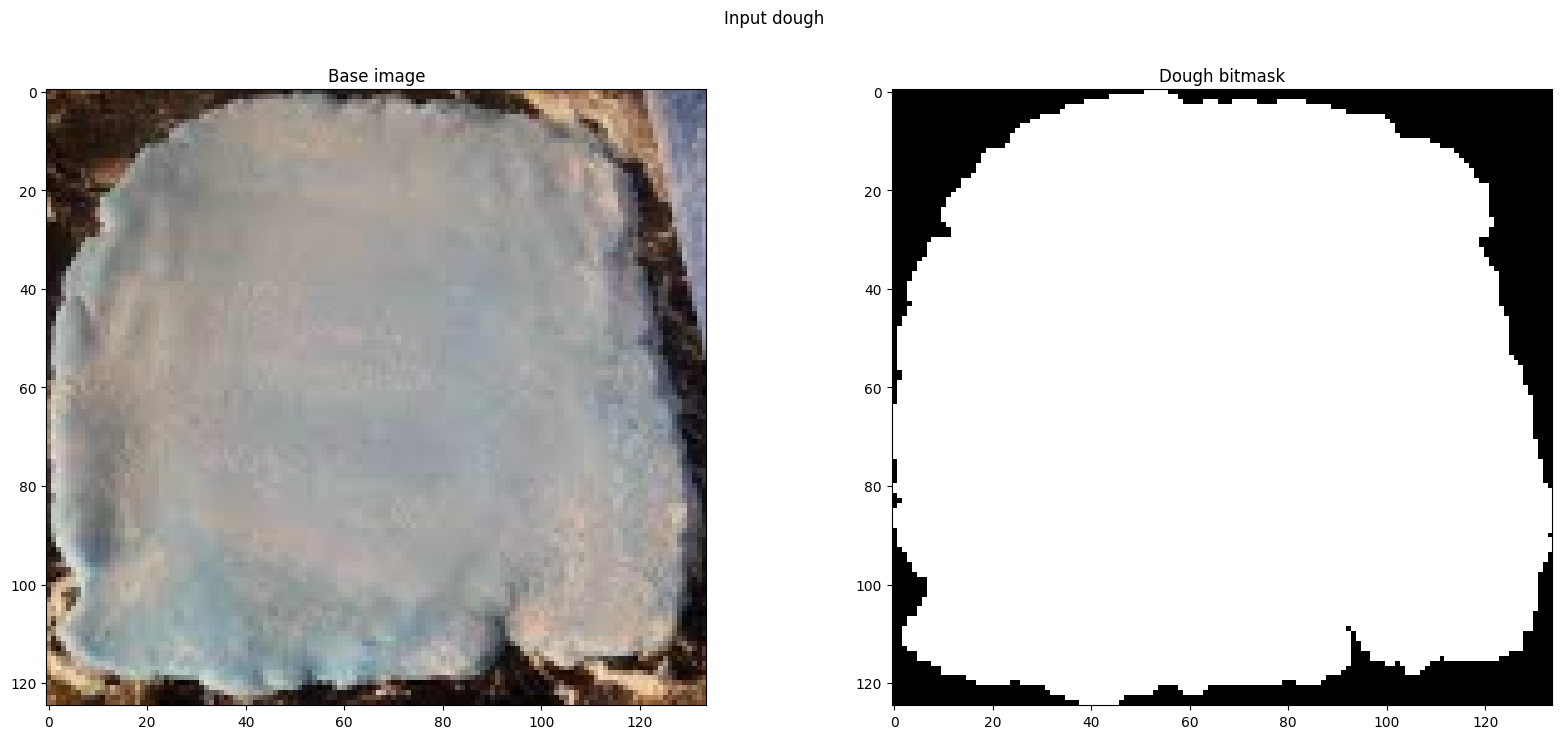
\includegraphics[width=\textwidth, keepaspectratio]{01-intro/subsampled_dough}
		\caption{Input dough and its binary mask (134×125 pixels)}
		\label{fig:input_dough}
	\end{subfigure}
	
	\begin{subfigure}{\textwidth}
		\centering	
		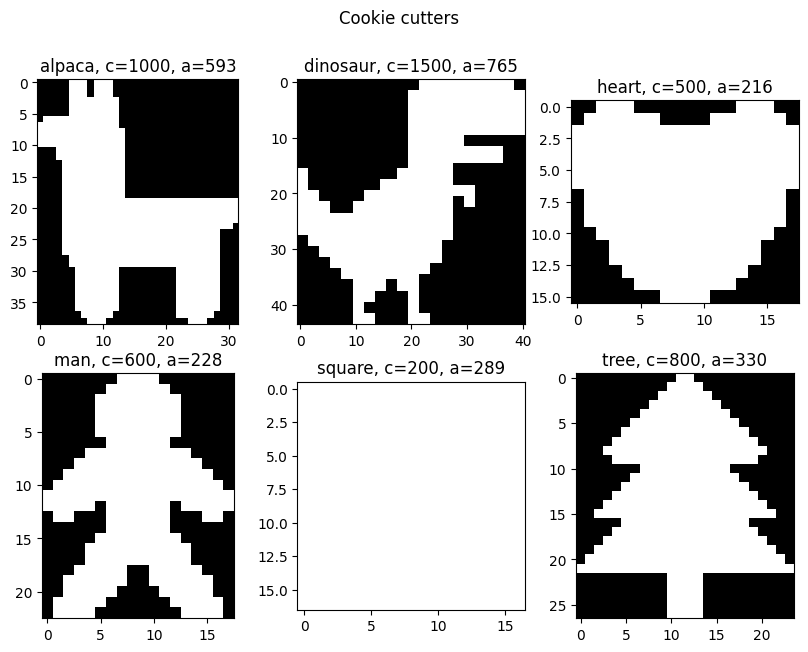
\includegraphics[width=.8\textwidth, keepaspectratio]{01-intro/cutters}
		\caption{Cutters' binary masks}
		\label{fig:cutters}
	\end{subfigure}
\end{figure}

\newpage

\subsection{Technology}
This project was developed with both AMPL and Jupyter Notebooks using the following technologies:
\begin{itemize}[itemsep=-1mm, topsep=0mm]
	\item AMPL with CPLEX solver
	\item Python with Google's OR-Tools optimization suite and CP-SAT solver
	\item Python with Gurobi's API and solver
	\item Pure Python for heuristics
\end{itemize}
All algorithms were run on a desktop setup with an Intel Core i7-6700 processor and 16GB DDR3 RAM; Python 3.9.12 was installed inside a Windows 10 Anaconda Environment. Only the nesting model with OR-Tools was run remotely on the Kaggle platform.

	
	% Optimization Project: Biscuit Optimizer
% Roberto Basla
% Politecnico di Milano
% A.Y. 2021/2022

\section{Modeling}
This section covers modeling approaches to the problem using AMPL, Google OR-Tools and Gurobi.

\subsection{Integer knapsack model}
The first approach consists in a relaxation of the problem that doesn't consider the placement of cutters on the dough: in this case only areas are considered, and the input image's mask $B$ is reduced to the number of available pixels (namely, $B = 13929$). Additional parameters are the cutter values $\underline{c}$ and cutter areas $\underline{a}$, while the integer vector $\underline{x}$ represents the number of times each cutter is selected (and is therefore the problem's variable).

This simpler problem consists in an integer knapsack that can be modeled as follows:
\begin{alignat}{3}
	\textrm{max}	&\quad& \sum_{i \in I}{c_i x_i}	& 				&& \label{eq:obj_knapsack} 		\\
	\textrm{s.t.}  	&\quad& \sum_{i \in I}{a_i x_i} & \leq B 		&& \label{eq:budget_knapsack} 	\\
					&\quad& x_i 					& \leq 3x_j		&& \quad \forall i \in I, \forall j \in I \label{eq:freq_knapsack} \\
					&\quad& x_i 					& \geq 0 		&& \quad \forall i \in I \label{eq:nonneg_knapsack} 
\end{alignat}

It maximizes the biscuit value multiplied by the number of times the cutter is used (\ref{eq:obj_knapsack}), subject to the knapsack's budget constraint (\ref{eq:budget_knapsack}) and the frequency constraints (\ref{eq:freq_knapsack}). Obviously, cutters must be selected a non-negative number of times (\ref{eq:nonneg_knapsack}).

As with any relaxation, the solution value is expected to be an upper bound for the complete problem.

\subsubsection{Results}
The model was solved very quickly by all three softwares, achieving a final value of $29000$ and a dough usage of 99.94\% of its pixels with the solution
$$
\underline{x} = 
\begin{bmatrix}
	4  \\
	4  \\
	4  \\
	11 \\
	4  \\
	12
\end{bmatrix}
$$

Figure \ref{fig:knapsack} shows the types of biscuits resulting from the optimization (39 in total). Models and results are available in the GitHub repository \href{https://github.com/rb-sl/biscuit_optimizer/tree/main/src/01-knapsack}{rb-sl/biscuit\_optimizer/src/01-knapsack}.

\begin{figure}[H]
	\centering	
	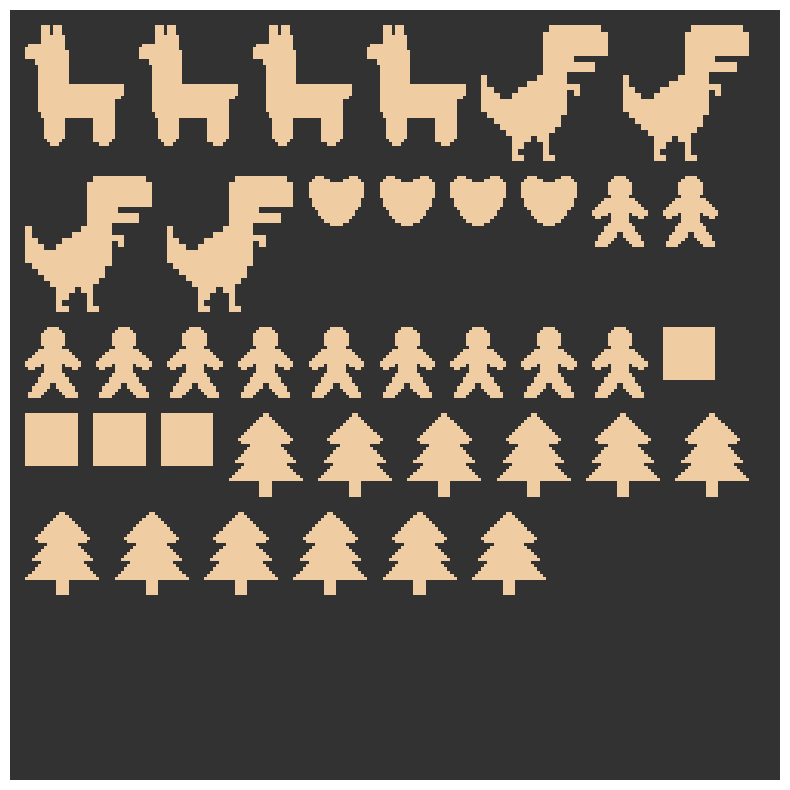
\includegraphics[width=.5\textwidth, keepaspectratio]{02-modeling/knapsack_visualization}
	\caption{Visualization of biscuits resulting from the knapsack problem}
	\label{fig:knapsack}
\end{figure}

\subsection{Nesting model}\label{sec:nesting}
The complete nesting model takes into account the initial mask and the cutter masks (so that they do not overlap). The solution is achieved through a set of binary variables $y$ over sets $I$ (the set of cutters), $N$ (the set of rows in the dough mask) and $M$ (the set of columns in the dough mask). $y_{i, n, m}$ is equal to 1 if a cutter $i$ is placed on the dough mask such that its top left corner is on the $(n, m)$ pixel in the mask.

In addition to sets and parameters already defined, the additional sets $\textrm{IN}_i$ and $\textrm{OUT}_i$ need to be defined as
\begin{alignat}{1}
	\textrm{IN}_i	& = \{(n, m): n \in N, m \in M, n + R_{i,max} \leq N_{max} \wedge m + C_{i,max} \leq M_{max} \} \notag \\
	\textrm{OUT}_i 	& = \{(n, m): n \in N, m \in M, n + R_{i,max} > N_{max} \vee m + C_{i,max} > M_{max} \} \notag
\end{alignat}
Naturally, it follows from the definition that $\textrm{IN}_i \cap \textrm{OUT}_i = \emptyset$ and $\textrm{IN}_i \cup \textrm{OUT}_i = B$, where $B$ represents the dough bitmask.
These sets need the additional parameters:
\begin{itemize}[itemsep=-1mm, topsep=0mm]
	\item $N_{max}$: number of rows of the dough mask
	\item $M_{max}$: number of columns of the dough mask
	\item $R_{i,max}$: number of rows of cutter $i$
	\item $C_{i,max}$: number of columns of cutter $i$
\end{itemize}
Figure \ref{fig:in_out} shows an example of these sets and parameters for $i=1$.

\begin{figure}[H]
	\centering	
	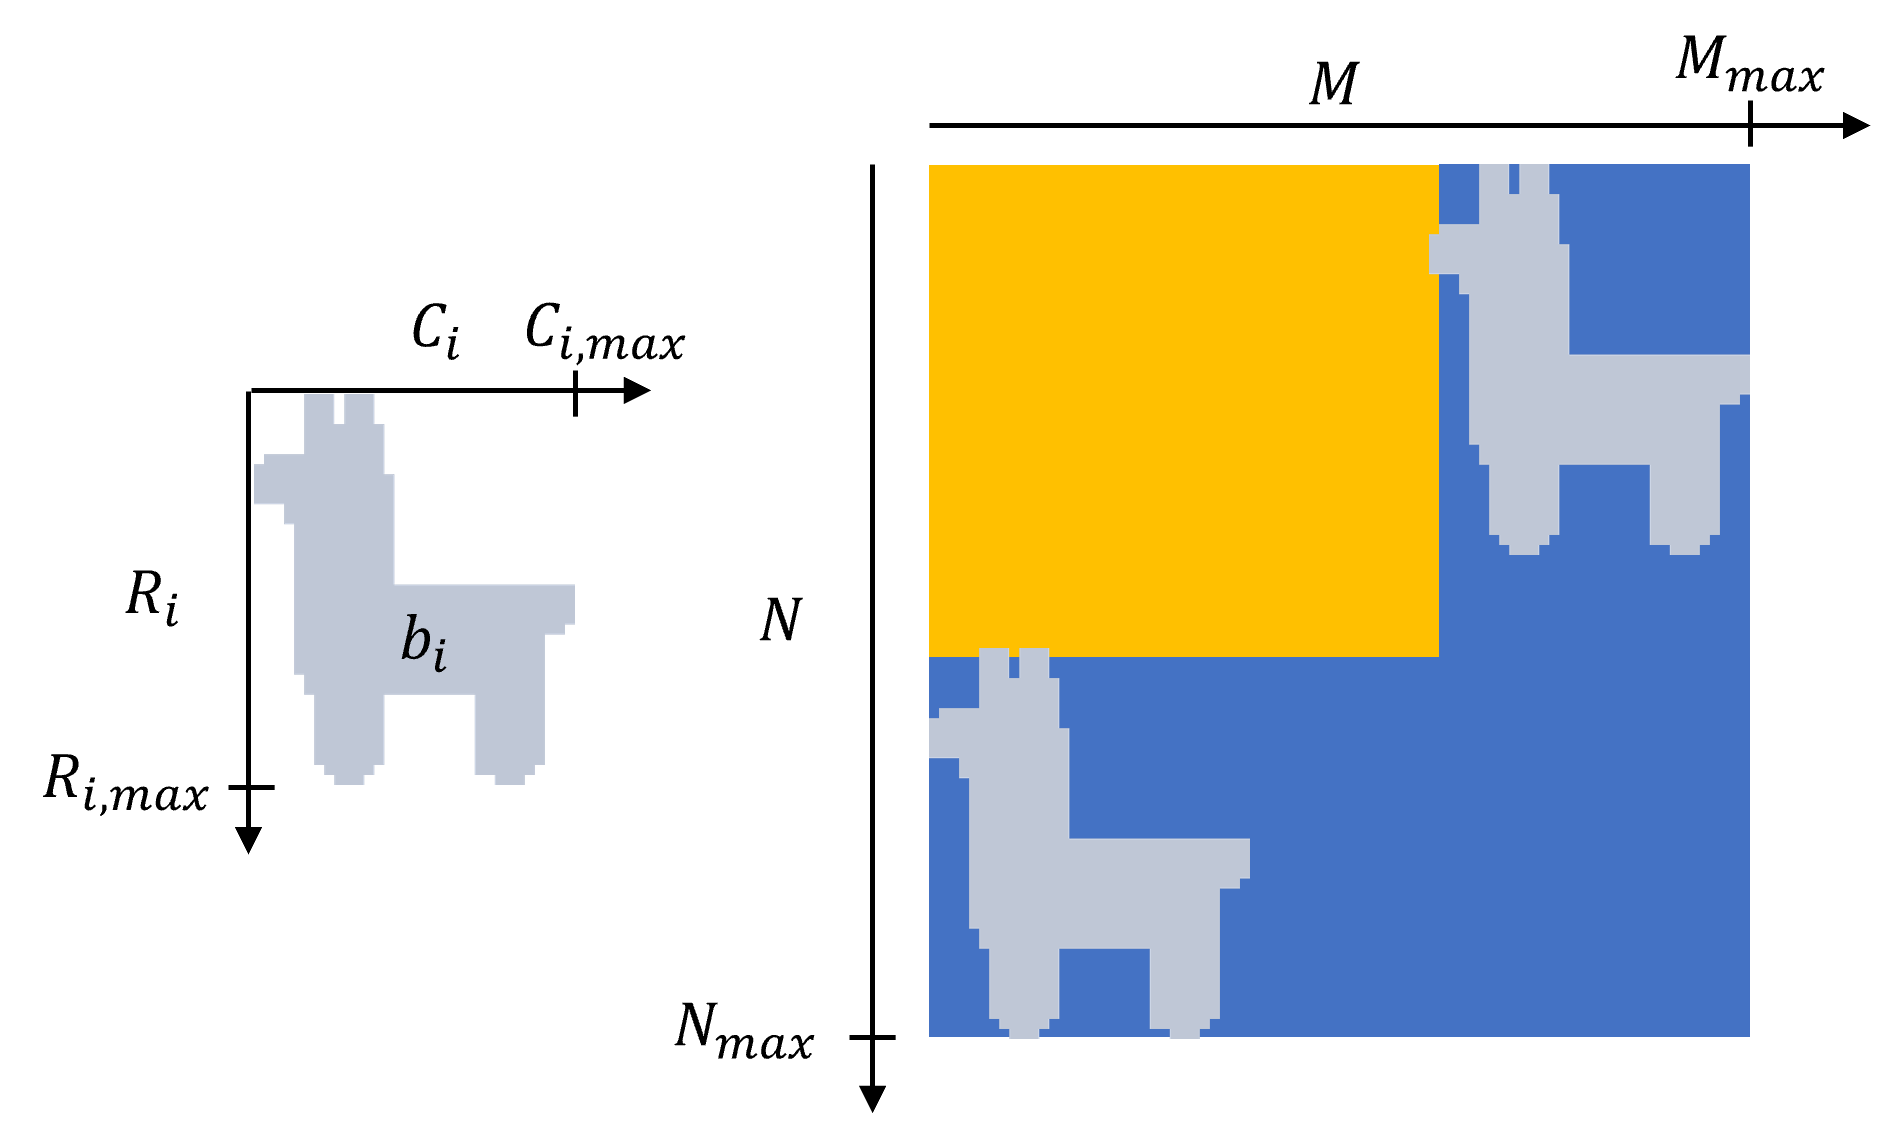
\includegraphics[width=.7\textwidth, keepaspectratio]{02-modeling/in_out}
	\caption{Examples of sets $\textrm{IN}_i$ (yellow) and $\textrm{OUT}_i$ (blue) for $i=1$}
	\label{fig:in_out}
\end{figure}

Finally, in order to help the formulation of the non-overlapping constraints, the integer variable $z$ is introduced over $I$, $N$ and $M$. $z_{i, n, m}$ represents the number of cutter masks $i$ that cover pixel $(n, m)$ (obviously, only the active part of a cutter mask influences $z$). Therefore, the complete nesting model is:
\begin{alignat}{3}
	\textrm{max}	& \sum_{i \in I}{c_i \sum_{n \in N}{\sum_{m \in M}{y_{i,n,m}}}} && \label{eq:obj_nest} \\
	\textrm{s.t.} \quad y_{i, n, m} & = 0 && \forall i \in I, \forall (n, m) \in \textrm{OUT}_i \label{eq:out_nest} \\
	y_{i, n, m} & \leq B_{n+h-1, m+k-1} + (1 - b_{i, h, k}) && \forall i \in I, \forall (n, m) \in \textrm{IN}_i, \notag \\
	& & & \forall h \in R_i, \forall k \in C_i \label{eq:in_nest} \\
	z_{i, n, m} & = \sum_{h \in R_i}{\sum_{k \in C_i}{y_{i,n-h+1, m-k+1}  b_{i, h, k}}} &\ & \forall i \in I, \forall n \in N, \forall m \in M \label{eq:link_nest} \\
	\sum_{i \in I}{z_{i, n, m}} & \leq 1 && \forall n \in N, \forall m \in M \label{eq:overlap_nest} \\
	\sum_{n \in N}{\sum_{m \in M}{y_{i,n,m}}} & \leq 3 \sum_{n \in N}{\sum_{m \in M}{y_{j,n,m}}} && \forall i \in I, \forall j \in I \label{eq:freq_nest} \\					
y_{i, n, m} & \in \{0, 1\} && \forall i \in I, \forall n \in N, \forall m \in M \label{eq:def_y} \\
z_{i, n, m} & \geq 0 && \forall i \in I, \forall n \in N, \forall m \in M \label{eq:def_z}
\end{alignat}

The objective function (\ref{eq:obj_nest}) is equivalent to the knapsack objective (\ref{eq:obj_knapsack}) (as $\sum_{n \in N}{\sum_{m \in M}{y_{i,n,m}}} = x_i \quad \forall i \in I$) and thus maximizes the overall value of chosen cutters. 

Constraint set (\ref{eq:out_nest}) enforces that the optimizer cannot place cutters that would result in partially cut-out biscuits due to the dough mask not being able to host them whole (thus operates on $\textrm{OUT}_i$); on the other hand, constraint set (\ref{eq:in_nest}) operates on the $\textrm{IN}_i$ sets and enforces that an $y_{i, n, m}$ may be selected only if the active pixels of cutter mask $i$ on $(n, m)$ fall on active pixels of the dough mask starting from $(n, m)$ up to $(n+R_i, m+C_i)$; it consists in the linearization of an AND operation. 

The set of linking constraints (\ref{eq:link_nest}) defines $z$ in function of $y$ so that the value of a $y_{i, n-h+1, m-k+1}$ (i.e., in the range defined by the cutter mask's dimension) is added to $z_{i, n, m}$ only if the cutter bitmask $b_{i, h, k}$ is active. Constraints (\ref{eq:overlap_nest}) enforce the non-overlapping property of the model by limiting the sum of active masks at each pixel $(n, m)$ in the dough mask.

Finally, constraints (\ref{eq:freq_nest}) enforce the maximum difference between the most frequently chosen cutter and the most infrequent. (\ref{eq:def_y}) and (\ref{eq:def_z}) define the variables.

\subsubsection{Results}
Due to the NP-Hard nature of the nesting problem, all solvers needed to be limited in time: the execution limit was set to 40000 seconds (some minutes less than 12 hours) for all instances. This decision may be the cause of the three optimizers finding different (locally optimal) solutions, unlike in the knapsack case where they were able to solve the problem exactly. It should be also noted that Python solutions added a small preprocessing, effectively merging constraints (\ref{eq:out_nest}) and (\ref{eq:in_nest}) in the form
\begin{lstlisting}[language=Python]
for i in I:
  for n in N:
    for m in M:
      if not can_host(dough_mask, cutter_mask, n, m):
        model.addConstr(y[n, m, i] == 0)
\end{lstlisting}
Effectively reducing the number of constraints by checking a priori with the \texttt{can\_host} function if a cutter $i$ could be placed in $(n, m)$ and, if not, just forcing $y_{i, n, m}$ to 0.

Models and results are available in the GitHub repository \\ \href{https://github.com/rb-sl/biscuit_optimizer/tree/main/src/02-nesting}{rb-sl/biscuit\_optimizer/src/02-nesting}.

\paragraph{AMPL solution}
The solution found by the CPLEX optimizer over the model defined in AMPL reached the objective of 16300 and is displayed in Figures \ref{fig:ampl_nest_overlay} and \ref{fig:ampl_nest_vis}.

\paragraph{OR-Tools solution} 
The CP-SAT optimizer solving the model defined in Google OR-Tools found a solution with value 17800, shown in Figures \ref{fig:ortools_nest_overlay} and \ref{fig:ortools_nest_vis}. Thanks to the possibility of adding callbacks every time a new solution is found, for this optimizer Figure \ref{fig:ortools_time} shows the plot of time against the best solution found. 

\paragraph{Gurobi solution}
Gurobi was able to reach the objective value of 17800 (using the same cutters) as well, but with a different configuration as shown in Figures \ref{fig:gurobi_nest_overlay} and \ref{fig:gurobi_nest_vis}.

\begin{figure}[H]
	\centering	
	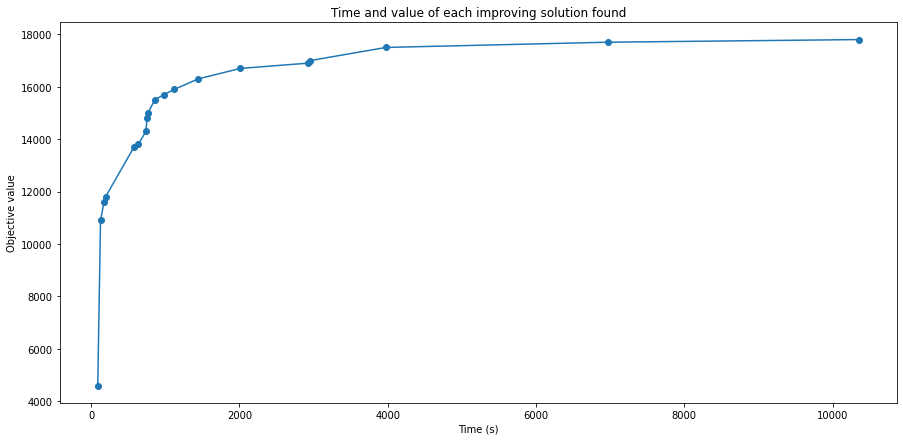
\includegraphics[width=\textwidth]{02-modeling/nest_ortools_time}
	\caption{Plot of the best current solution found by CP-SAT against time}
	\label{fig:ortools_time}
\end{figure}

\begin{figure}[p]
	\begin{subfigure}[b]{.43\textwidth}
		\centering
		\fbox{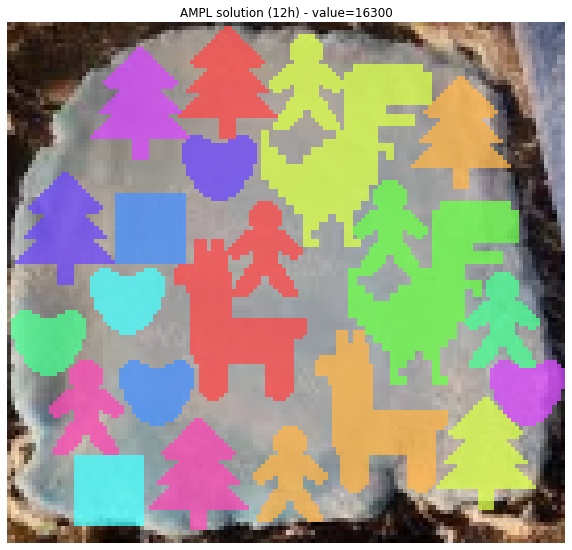
\includegraphics[width=\textwidth]{02-modeling/nest_ampl_overlay}}
		\caption{AMPL/CPLEX solution}
		\label{fig:ampl_nest_overlay}
	\end{subfigure} 
	\hfill
	\begin{subfigure}[b]{.43\textwidth}
		\centering
		\fbox{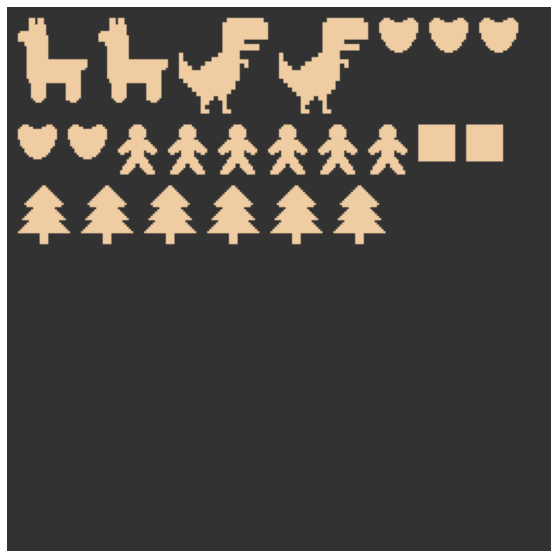
\includegraphics[width=\textwidth]{02-modeling/nest_ampl_visualization}}
		\caption{AMPL biscuits result}
		\label{fig:ampl_nest_vis}
	\end{subfigure}

	\vfill
	
	\begin{subfigure}[b]{.43\textwidth}
		\centering
		\fbox{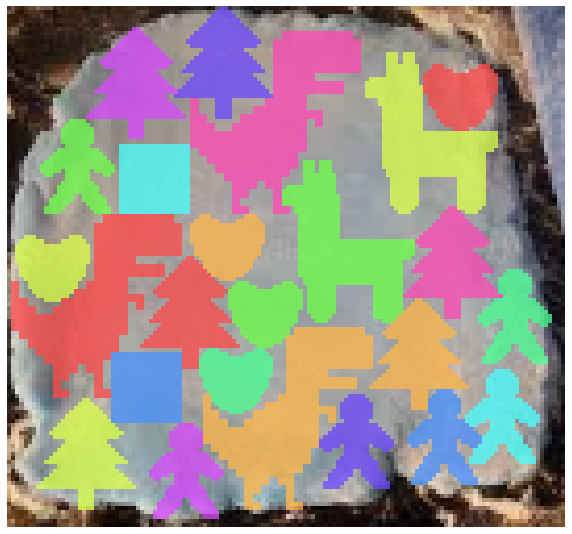
\includegraphics[width=\textwidth]{02-modeling/nest_ortools_overlay}}
		\caption{OR-Tools/CP-SAT solution}
		\label{fig:ortools_nest_overlay}
	\end{subfigure} 
	\hfill
	\begin{subfigure}[b]{.43\textwidth}
		\centering
		\fbox{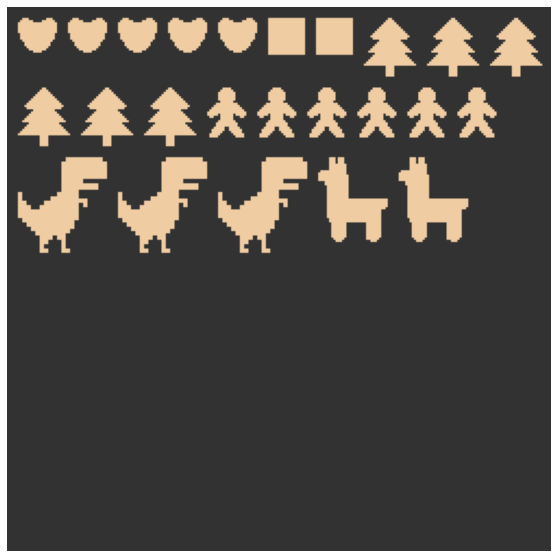
\includegraphics[width=\textwidth]{02-modeling/nest_ortools_visualization}}
		\caption{OR-Tools biscuits result}
		\label{fig:ortools_nest_vis}
	\end{subfigure}

	\vfill
	
	\begin{subfigure}[b]{.43\textwidth}
		\centering
		\fbox{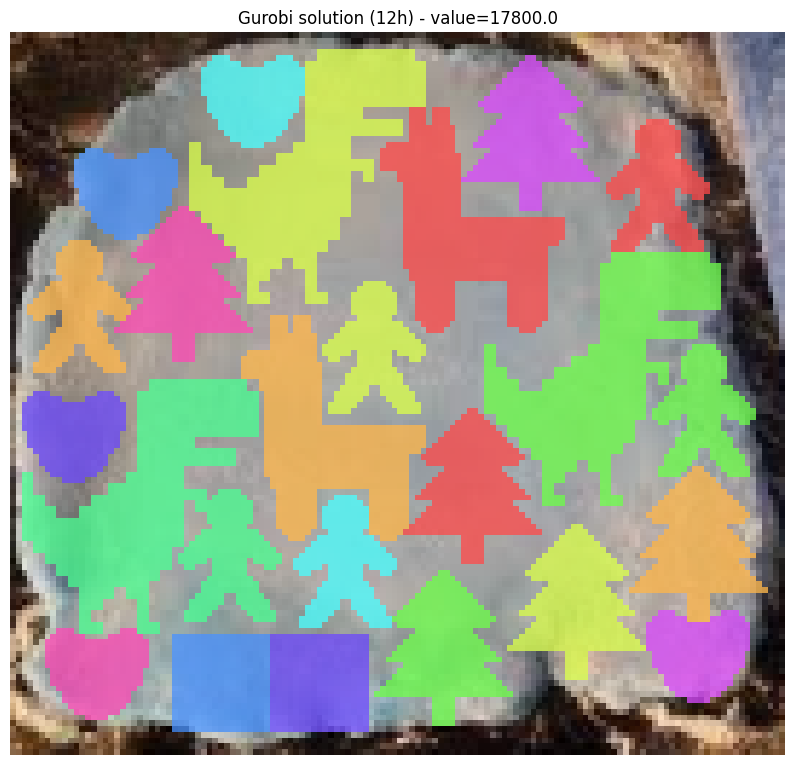
\includegraphics[width=\textwidth]{02-modeling/nest_gurobi_overlay}}
		\caption{Gurobi solution}
		\label{fig:gurobi_nest_overlay}
	\end{subfigure} 
	\hfill
	\begin{subfigure}[b]{.43\textwidth}
		\centering
		\fbox{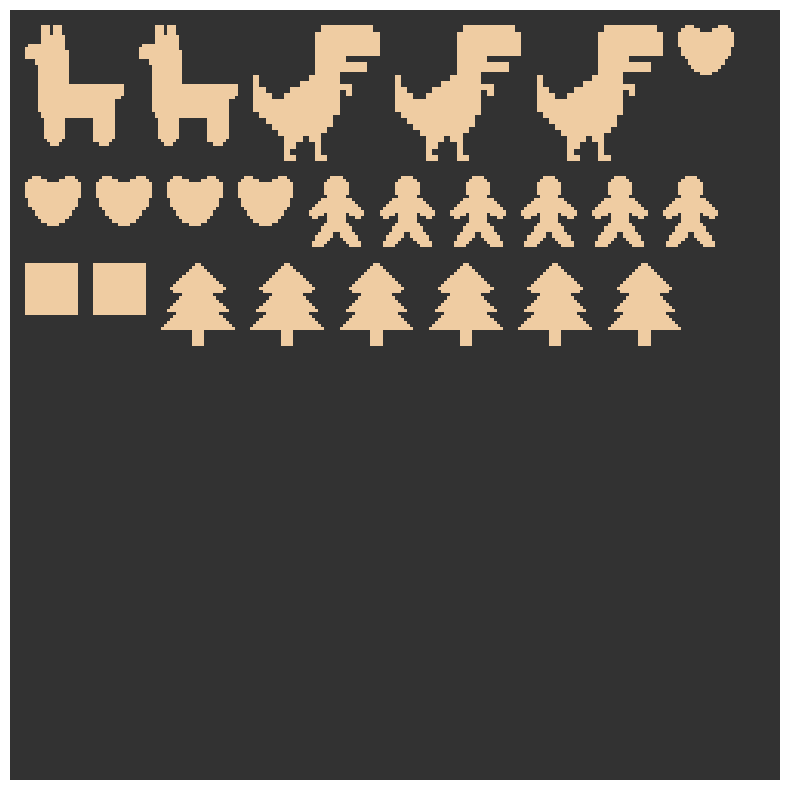
\includegraphics[width=\textwidth]{02-modeling/nest_gurobi_visualization}}
		\caption{Gurobi biscuits result}
		\label{fig:gurobi_nest_vis}
	\end{subfigure}
	\caption{Nesting results}
	\label{fig:nesting_results}
\end{figure}

	
	% Optimization Project: Biscuit Optimizer
% Roberto Basla
% Politecnico di Milano
% A.Y. 2021/2022

\section{Heuristic solutions}\label{sec:heuristics}
As the solvers were not able to find a solution in a reasonable time, some heuristics were devised to tackle the problem. Python notebooks ot the experiments are available in the GitHub repository  \href{https://github.com/rb-sl/biscuit_optimizer/tree/main/src/03-heuristics}{rb-sl/biscuit\_optimizer/src/03-heuristics}.

\subsection{Greedy heuristics}\label{sec:greedy}
The first set of heuristics tries to solve the nesting problem greedily. In order to do so, a series of cost map encoding the cost of activating a variable \texttt{y[i, n, m]} (i.e., placing a cutter of type $i$ at coordinates $(n, m)$) was defined:
\begin{itemize}[itemsep=-1mm, topsep=0mm]
	\item Value-based cost map: assigns the cost $c_{i,n,m} = -v_i$ (i.e. the negative value of cutter $i$) to each \texttt{y[i, n, m]} independently of the position $(n, m)$
	\item Area-based cost map: assigns the cost $c_{i,n,m} = a_i$ (i.e. the area consumption of cutter $i$) to each \texttt{y[i, n, m]} independently of $(n, m)$
	\item Occupancy-based cost map: assigns to each \texttt{y[i, n, m]} a cost proportional to the number of \texttt{y} variables that would be made infeasible by activating \texttt{y[i, n, m]} at the first step, $c_{i, n, m} = \textrm{len}(o_{i, n, m})$ with $o$ representing the list of $y$s made infeasible by each $(i, n, m)$
	\item Composition of Value and Area cost maps: $c_{i, n, m} = -\frac{v_i}{a_i}$
	\item Composition of Value and Occupancy cost maps: $c_{i, n, m} = -\frac{v_i}{o_{i, n, m} + 1}$
	\item Composition of Area and Occupancy cost maps: $c_{i, n, m} = (o_{i, n, m} + 1) \cdot a_i$
\end{itemize}
These cost maps define the quantities to be minimized by the greedy procedures, while the actual results refer to the sum of biscuit values. 

\subsubsection{Results}
Heuristics were run 100 times to find average results for each strategy. Figure \ref{fig:heuristics_results} shows their distribution: only strategies involving the occupancy were consistent in their results, as that was the only cost map that defined values for $(i, n, m)$ instead of for $i$ only. Other heuristics had intrinsic randomness, either explicitly defined (as in the case of greedy/random) or implicitly (e.g., the area case would be greedy only in choosing the cutter and random in selecting the position).

Table \ref{tab:heuristics_results} reports average values and time for the simulations; it introduces a completely random baseline to compare the results. In general, results were worse than the ones provided by complete nesting models; in particular, heuristics including areas performed worse than the other cases (area-based only was even worst than the random baseline). The best performing strategy (greedy combining value and occupancy) is kept for the next section.

\begin{center}
	\begin{tabular}{r|c|c}
		Heuristic					& Average value	& Time for 100 simulations (s) 	\\
		\hline
		Random (baseline) 			& 9151 			& 277.8 						\\
		Greedy/Random 				& 13489 		& 331.79 						\\
		Greedy (value) 				& 13249			& 334.69 						\\
		Greedy (area) 				& 9000 			& 260.93						\\
		Greedy (occupancy) 			& 15600			& 329.51						\\
		Greedy (value+area) 		& 9555			& 258.44						\\
		Greedy (value+occupancy)	& 16900			& 353.11						\\
		Greedy (area+occupancy)		& 15600			& 378.72						\\
	\end{tabular}
	\captionof{table}{\label{tab:heuristics_results}Heuristics results}
\end{center}

\begin{figure}[H]
	\centering	
	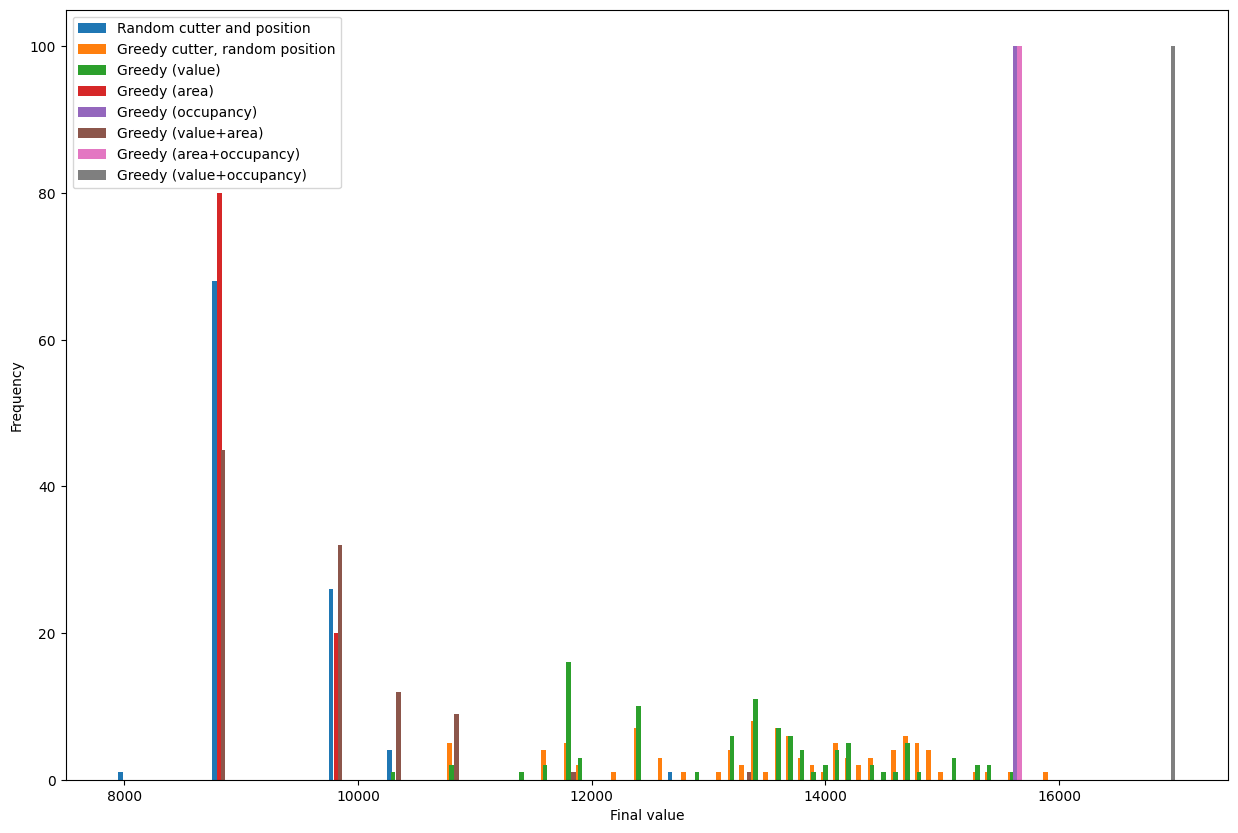
\includegraphics[width=\textwidth]{03-heuristics/heuristic_simulations}
	\caption{Distribution of heuristic results over 100 simulations for each strategy}
	\label{fig:heuristics_results}
\end{figure}

\subsection{GRASP}
The last class of implemented heuristics is Greedy Randomized Adaptive Search Procedures as described by Resende and Ribeiro\cite{grasp}. It is composed of two main phases that are iterated a number of times.

\paragraph{Greedy Randomized Construction} This phase builds a solution by first creating a Restricted Candidate List (RCL) containing elements with the smallest incremental cost as defined by the cost map. Elements $e = (i, n, m)$ are chosen to be part of the RCL if their cost $c(e)$ is
$$
c(e) \in [c^{min}, c^{min} + \alpha (c^{max} - c^{min})]
$$ 
For some choice of $\alpha$. The next element is chosen randomly from the RCL.

\paragraph{Local search} This phase searches the neighborhood of the solution found by the previous phase as in Hill Climbing. The neighborhoods are built according to the scheme defined by Delorme et al.\cite{local_search} using k-p exchanges, which consist in varying k variables from 1 to 0 and p variables from 0 to 1. In particular were used 0-1, 1-1, 1-2 and 2-1 exchanges.

\vspace{20px}

While previous heuristics encoded solutions as human-readable Python dictionaries, results are now encoded as 3D NumPy arrays of shape $n_{cutters} \times n_{rows} \times n_{columns}$ that correspond to variables $y$ in Section \ref{sec:nesting}:
\begin{equation}\notag
	y_{i, n, m} = 
	\begin{cases}
		1 \quad \textrm{if the solution has a cutter } i \textrm{ in position } (n, m) \\
		0 \quad \textrm{otherwise}
	\end{cases}
\end{equation}
With this definition, the symmetric distance becomes just
$$
\Delta(s, g) = \sum_{i \in I}\sum_{n \in N}\sum_{m \in M} |s_{i, n, m} - g_{i, n, m}|
$$
i.e. the number of different elements between the starting solution $s$ and the guiding solution $g$.

This project's implementation made some changes with respect to the paper's description, namely:
\begin{itemize}[itemsep=-1mm, topsep=0mm]
	\item The Greedy Randomized Construction phase doesn't stop in order to avoid impeding the construction of a feasible solution with the remaining cutters for performance purposes: this change improved the construction time to 2s from 21s (on average) without impacting the quality of solutions
	\item The Greedy Randomized Construction phase doesn't build infeasible solutions, so the repair procedure is not needed
	\item The Local Search used two additional parameters limiting the maximum total time and the maximum time between improvements, as the neighborhood exploration is the slowest phase (even if it can be faster when starting from a good solution\cite{local_search})
\end{itemize}

\subsubsection{Path Relinking}
Path Relinking aims at exploring trajectories connecting solutions obtained by the GRASP procedure. It keeps an elite pool of the best solutions found and relinks them to new GRASP solutions, potentially obtaining better results. The choice of which (initial) solution is relinked to the other (guiding) determines the type of Path Relinking. This project implements the following alternatives, as described in \cite{grasp}:
\begin{itemize}[itemsep=-1mm, topsep=0mm]
	\item Forward Path Relinking: the GRASP output is the initial solution while the guiding solution is chosen from the elite pool according to its distance
	\item Backward Path Relinking: the roles of initial and guiding solutions are inverted with respect to the previous case
	\item Mixed Path Relinking: the origin of the two solution is changed at each iteration
	\item Evolutionary Path Relinking: every $e$ steps of any of the previous variants the solutions in the elite pool are relinked among themselves
\end{itemize}
The only changes with respect to the algorithm description in the paper were the addition of a tabu list to the local search phase containing the initial and guiding solutions (otherwise many solutions tend to fall back into local optima found by GRASP), and limiting the minimum distance of new elite solutions when the pool is not full as well.

\subsubsection{Results}
GRASP and its Path Relinking variant were able to consistently reach and exceed the values obtained by nesting models of section \ref{sec:nesting}. Table \ref{tab:grasp_results} contains the best results for each of the implemented strategies.

\paragraph{GRASP} GRASP heuristics were run 100 times to assess the average value of solutions, which is close to that of the best heuristic in Section \ref{sec:greedy} (being 16834, obtained in 17315.07s). However, it was able to reach higher values as shown in Figure \ref{fig:grasp_100}, and considering that GRASP's result are actually given by the best one among a number of iterations (instead of just one as in the test), it is able to consistently outperform the previously considered heuristics. An example using 5 iterations is reported in Table \ref{tab:grasp_results}.

\paragraph{Path Relinking} Path Relinking proved to be a good enhancement: the following output shows an example where solutions with values 16900 and 17900 generated a solution with value 17400 (the best one along the path), which led to the best solution after local search.

\begin{footnotesize}
	\begin{verbatim}
		PATH RELINKING: 6/10
		GRASP: 1/3
		Starting local search from solution v=15900
		Best solution after local search (5 improvements / 13095 checked): v=16900
		GRASP: 2/3
		Starting local search from solution v=15300
		Best solution after local search (5 improvements / 19186 checked): v=16100
		GRASP: 3/3
		Starting local search from solution v=15400
		Best solution after local search (4 improvements / 18033 checked): v=16400
		>>> [17900, 17500, 17900, 17200, 17900]
		Starting relinking of solution v=16900 to v=17900 (distance = 40.0)
		Best relinking solution in path (40 steps / 328 checks): v=17400 at step=39
		Best solution after local search (2 improvements / 2335 checked): v=18300
	\end{verbatim}
\end{footnotesize}
An example of Path Relinking and Local Search is displayed in Figure \ref{fig:path_relinking}. This enhancement was not tested for 100 steps as the output is not independent from previous iterations. However, it was able to find a better solution than the Python models with value 18500 (shown in Figure \ref{fig:pr_18500}). 

Finally, the following output shows an example of successful evolution, where the new elite pool consists in the result for \texttt{k=4}:
\begin{footnotesize}
	\begin{verbatim}
		k=1: [16800,17100,16900]             => [17300,16900,16800,17000,16600]
		k=2: [17300,16900,16800,17000,16600] => [17200,17500,17500,17600,17500]
		k=3: [17200,17500,17500,17600,17500] => [17900,17600,17800,17600,17500]
		k=4: [17900,17600,17800,17600,17500] => [17800,17900,17800,17800,17700]
	\end{verbatim}
\end{footnotesize}

\begin{figure}[p]
	\centering
	\begin{subfigure}[b]{.49\textwidth}
		\centering
		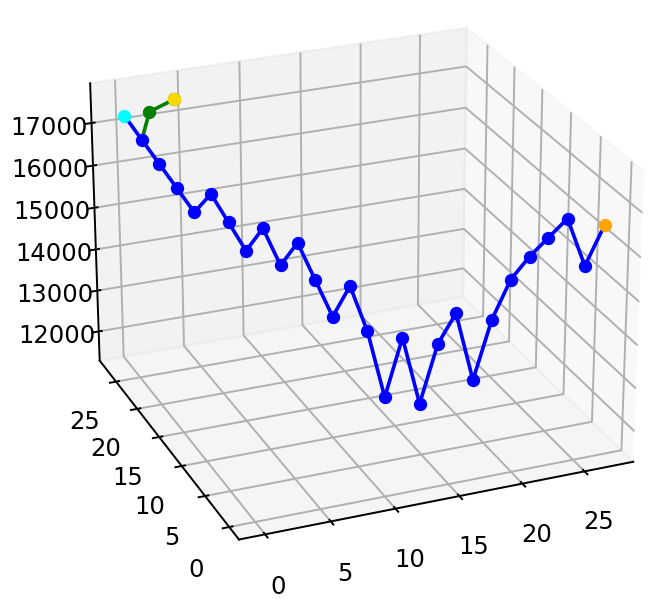
\includegraphics[width=\textwidth]{03-heuristics/paths/cut_pr_over}
		\caption{3D Path Relinking plot}
		\label{fig:pr_over}
	\end{subfigure}
	\hfill
	\begin{subfigure}[b]{.49\textwidth}
		\centering
		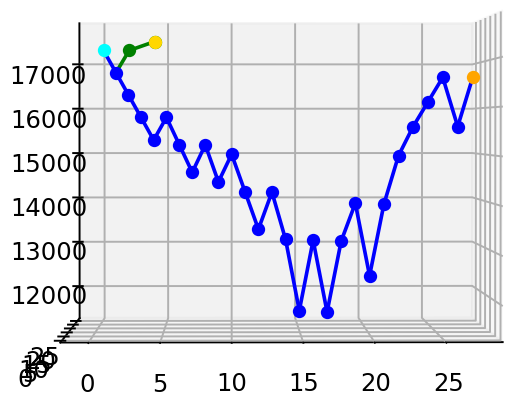
\includegraphics[width=\textwidth]{03-heuristics/paths/cut_pr_v_start}
		\caption{Projection over distance from the starting solution and value}
		\label{fig:pr_v_start}
	\end{subfigure}
	\caption{Path Relinking plot. Shows the starting solution (cyan), the guiding solution (orange) and the relinking path (blue). The Local Search path is in green, while the best final solution is gold. Axes correspond to distance from the starting solution, distance from the guiding solution and value.}
	\label{fig:path_relinking}
\end{figure}

\begin{figure}[p]
	\centering
	\begin{subfigure}[b]{.49\textwidth}
		\centering
		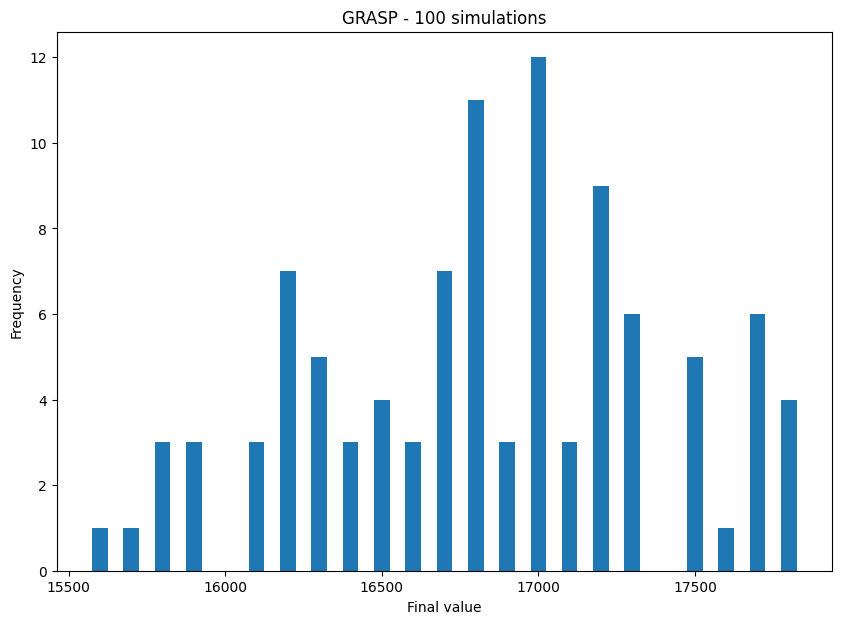
\includegraphics[width=\textwidth]{03-heuristics/grasp_100}
		\caption{100 single GRASP iterations}
		\label{fig:grasp_100}
	\end{subfigure}
	\hfill
	\begin{subfigure}[b]{.49\textwidth}
		\centering
		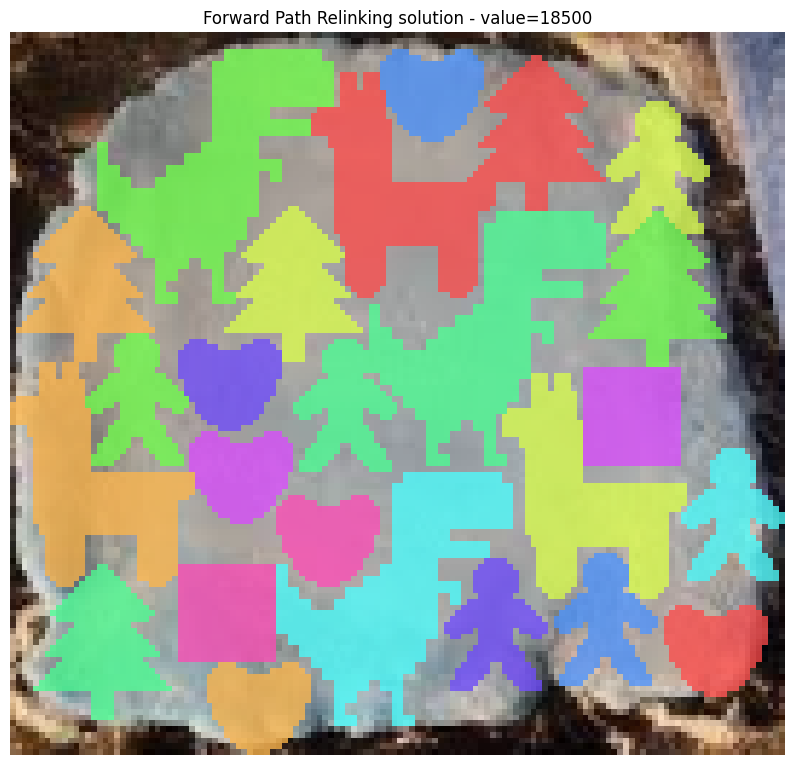
\includegraphics[width=\textwidth]{03-heuristics/pr_18500}
		\caption{Best Path Relinking solution}
		\label{fig:pr_18500}
	\end{subfigure}
	\label{fig:grasp_results}
	\caption{GRASP results}
\end{figure}

\vspace{20px}

\begin{center}
	\begin{tabular}{r|c|c|c}
		Heuristic							& Best value	& Iterations	& Time (s)	\\
		\hline
		GRASP 								& 17800			& 5				& 317.77	\\
		Forward Path Relinking				& 18500 		& 10 			& 2765.12	\\
		Backward Path Relinking				& 18300			& 10  			& 2761.82	\\
		Mixed Path Relinking 				& 18300			& 10	 		& 2776.01	\\
		Evolutionary Mixed Path Relinking	& 18300			& 20			& 9687.86	\\
	\end{tabular}
	\captionof{table}{\label{tab:grasp_results}GRASP and Path Relinking results}
\end{center}

	
	% Optimization Project: Biscuit Optimizer
% Roberto Basla
% Politecnico di Milano
% A.Y. 2021/2022

\section{Further applications: Histological images augmentation}

\subsection{The problem}

\subsection{Heuristic examples}


	
	% Optimization Project: Biscuit Optimizer
% Roberto Basla
% Politecnico di Milano
% A.Y. 2021/2022

\section{Conclusions}
	
	
	\bibliographystyle{plain}
	\bibliography{06-bibliography}	
\end{document}
